\documentclass[aps,letterpaper,11pt]{revtex4}
\usepackage{graphicx} % For images
\usepackage{float}    % For tables and other floats
\usepackage{verbatim} % For comments and other
\usepackage{amssymb}  % For more math
\usepackage{fullpage} % Set margins and place page numbers at bottom center
\usepackage{listings} % For source code
\usepackage[usenames,dvipsnames]{color} % For colors and names
\usepackage[pdftex]{hyperref}           % For hyperlinks and indexing the PDF
\usepackage{pdfpages}
\usepackage{subfig}
\usepackage{listings}
\usepackage[usenames,dvipsnames,svgnames,table]{xcolor}
\usepackage{color}
\usepackage{textcomp}
\usepackage[utf8]{inputenc}
% Custom colors
\definecolor{deepblue}{rgb}{0,0,0.5}
\definecolor{deepred}{rgb}{0.6,0,0}
\definecolor{deepgreen}{rgb}{0,0.5,0}

 \lstset{
  tabsize=4,
  language=C++,
  captionpos=b,
  tabsize=3,
  numberstyle=\tiny,
  numbersep=5pt,
  breaklines=true,
  showstringspaces=false,
  basicstyle=\footnotesize,
%  identifierstyle=\color{magenta},
  keywordstyle=\color[rgb]{0,0,1},
  commentstyle=\color{deepgreen},
  stringstyle=\color{deepred}
  }
  
\hypersetup{ % play with the different link colors here
    colorlinks,
    citecolor=black,
    filecolor=black,
    linkcolor=black,
    urlcolor=blue % set to black to prevent printing blue links
}

\newcommand{\labno}{Software Engineering Project}
\newcommand{\labtitle}{Weekly report}
\newcommand{\authorname}{Mladen Rakic}
\newcommand{\professor}{Dr. Yohan Fougerolle}


\begin{document}  
\begin{titlepage}
\begin{center}
{\LARGE \textsc{\labno:} \\ \vspace{4pt}}
{\Large \textsc{\labtitle} \\ \vspace{4pt}} 
\rule[13pt]{\textwidth}{1pt} \\ \vspace{150pt}
{\large By: \authorname \\ \vspace{10pt}
Professor: \professor \\ \vspace{10pt}
\today}
\end{center}


\end{titlepage}% END TITLE PAGE %%%%%%%%%%%%%%%%%%%%%%%%%%%%%%%%%%
\newpage
\section {Accomplished tasks}
From tomorrow I will not be in Le Creusot, which is the reason why my weekly report came early this week. This is the brief list of things I have managed to accomplish up to this point:\\
\linebreak
1. The GUI design has reached its final version. I added some new functionalities to it, such as the combo box to choose the registration method, button to enable filtering, list views to show point clouds. I also removed the logger from the scan window and left only the one in the main window, since the former was redundant.\\ 
\linebreak 
2. At this point, it is possible to load a point cloud into the GUI, as well as to display it in QVTK Widget. I managed to enable this with Antoine's help. One example of a loaded point cloud can be seen in figure 1. \\ 
\linebreak

\begin{figure}[!htb]
  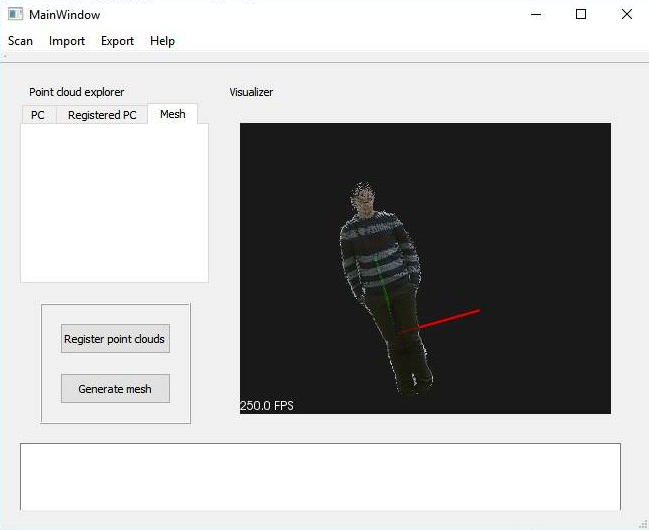
\includegraphics[scale=0.5]{mainwindow.png}
  \caption{Point cloud display}
  \label{fig:Kinect2}
\end{figure}


3. I was also present when Marcio was working on the logger class and I offered my help and support.\\
\pagebreak

\section {Future tasks}
My next weekly report will also be my last, so here I present the list of some of the final tasks that I have to complete:\\
\linebreak
1. One important thing to enable for the GUI is to display the list of the loaded point clouds in the tab widget. I will try to accomplish this task as quickly as possible, since it is needed for other members of the group, in order for them to be able to proceed with some of their challenges. For now I managed to create a function that might work, but it is still to be tested.\\
\linebreak
2. After I return, I will work with Marcio on visualization of the live scan and on the bounding box for the scan, which is possibly the last major task I will tackle.\\

\end{document} % DONE WITH DOCUMENT!

